\section{Design of CAPS}
\label{sec:design}

Following an overview of \ac{name}'s design (\autoref{sec:design:overview}), we
describe \ac{name} in detail, including how it signals which domains have
deployed \ac{https} and improvements to the Web \ac{pki}
(\autoref{sec:design:signaling}), how it provides stronger public-key
authentication over the existing Web \ac{pki} (\autoref{sec:design:policy}), and
how clients establish secure end-to-end connections with servers
(\autoref{sec:design:handshake}). We conclude by describing how \ac{name} thus
enables the bootstrapping of more advanced policies
(\autoref{sec:design:bootstrapping}).

\subsection{Overview}
\label{sec:design:overview}

\begin{figure*}
  \centering
  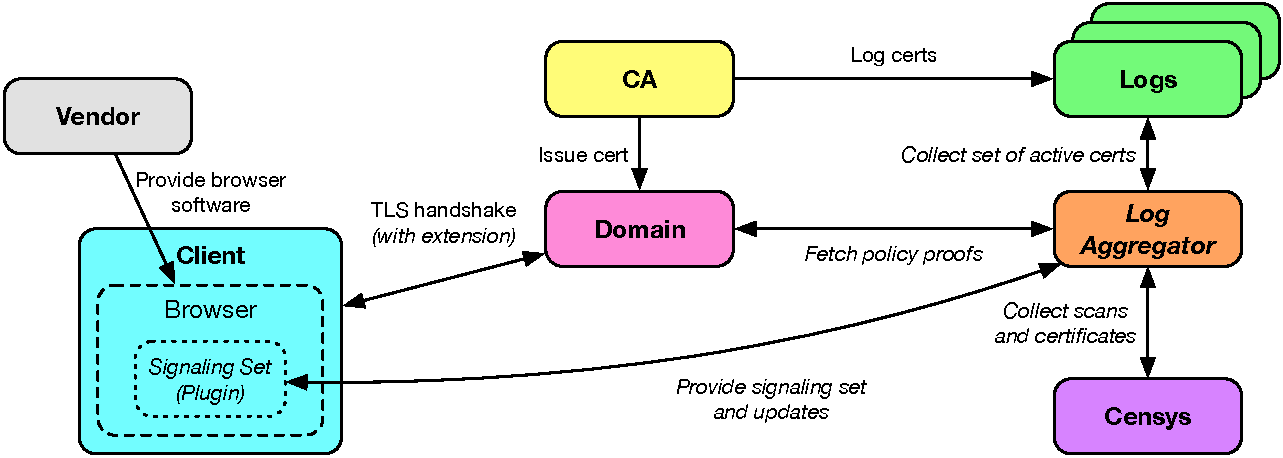
\includegraphics[width=0.8\linewidth]{fig/overview2}
  \caption{Overview of \ac{name} architecture (log auditors and monitors not
  shown). Dotted lines denote the browser and its components, and italic text
denotes new entities or actions in \ac{name}.}
  \label{fig:overview}
\end{figure*}

\paragraph{Goals}

\ac{name} primarily aims to enable a smooth transition from the Web's existing
\ac{pki} to an \emph{improved \ac{pki}} (which can range from an extension to
the existing \ac{pki} to a new \ac{pki} altogether). We assume that during this
transition, both the existing and improved \acp{pki} will coexist, and that the
improved \ac{pki} will make \ac{mitm} attacks more difficult to carry out.
Hence, \ac{name} must prevent downgrades to the old \ac{pki}. More precisely, if
a client and server both support the improved \ac{pki}, then when they perform a
handshake, they should negotiate a session key based on the domain's public key
as certified in the improved \ac{pki}. As secondary objectives, we also seek to
prevent domains from becoming inaccessible due to misconfiguration, private key
loss, or private key compromise, and to minimize the changes to existing
interactions between clients, domains, and \acp{ca}.

\paragraph{Adversary Model}

In designing \ac{name}, we consider an adversary with the goal of successfully
mounting \iac{mitm} attack. We assume that the adversary has access to the
signing keys for $n$ \acp{ca} and can thus issue and revoke arbitrary
certificates under these keys. We also assume that the adversary has full
control of the network during the handshake protocol; that is, the adversary can
intercept, drop, or modify all messages sent among all entities described
below. We assume that the adversary cannot mount \iac{mitm} in the improved
\ac{pki}, or break standard cryptographic primitives.

\paragraph{Architecture}

\autoref{fig:overview} illustrates the \ac{name} architecture and how \ac{name}
achieves the goals stated above. Since \ac{name} transitions from the current
Web \ac{pki}, it necessarily includes the entities in the current \ac{pki}:
\begin{compactitem}
\item \emph{Domains} serve webpages to clients. Each domain has a name such as
  \texttt{example.com}.
\item \emph{\acp{ca}} issue certificates to domains. Each certificate binds a
  set of names to a single public key.
\item \emph{Clients} connect to domains over HTTP or \ac{https}, and in the
  latter case, verify the binding between a domain's name and public key.
\item \emph{Browser/OS vendors} (hereafter simply \emph{vendors}) provide the
  software by which clients connect to domains and verify domains' certificates.
\item \emph{Public logs} maintain a publicly auditable, append-only database of
  certificates, such as those used in \ac{ct}.
\end{compactitem}
\ac{name} introduces a new entity, the \emph{log aggregator}, that uses publicly
available data to maintain a database of domains that have deployed \ac{https}
and/or the improved \ac{pki}. While we present the log aggregator as an
independent entity, in \autoref{sec:discussion} we argue that browser vendors
should take on this responsibility.

% Procedures from the current PKI
As shown in \autoref{fig:overview}, many of the interactions between entities in
the current \ac{pki} remain the same in \ac{name}. \acp{ca} issue certificates
to domains and log newly-issued certificates as they do in the current \ac{pki}
(with \ac{ct}); clients and domains establish an encrypted communication channel
through the \ac{tls} handshake, and vendors provide clients with browser
software.

% Signaling set overview
To prevent an adversary from forcing an HTTP connection (thus bypassing \ac{tls}
completely), the log aggregator uses data from public logs to construct a
\emph{signaling set}, which succinctly represents the set of all domains that
deploy \ac{https}. The log aggregator builds this set by downloading the set of
all currently valid (i.e., non-expired) certificates from the logs and
extracting all domains named in these certificates. The log aggregator then
makes this set, as well as updates to this set over time, available to client
browsers. With the signaling set, a browser making a request to a server can
first check whether or not the server has deployed \ac{https}.

% Policy overview
To allow domains to certify their public keys more securely than in the old
\ac{pki}, the log aggregator uses data from public logs to construct a set of
\emph{\ac{name} policies}, which establishes for each \ac{https}-deploying
domain one or more public keys to be treated as authoritative in the improved
\ac{pki}. To provide a smooth transition from the current \ac{pki}, \ac{name}
uses a simple, intuitive policy to determine a domain's public key in the
improved \ac{pki}: \emph{treat whichever public key is backed by the most
  independent certificate chains\footnote{This term means that the certificate
chains share no public keys except at the leaf.} in the current \ac{pki} as
authoritative in the improved \ac{pki}}. A domain wanting to increase client
confidence in one of its public keys can then simply obtain more independent
certificates for that key, and the log aggregator will update its key policy for
that domain.

Intuitively, the log aggregator simply sends a signed pair $(\hostname,
\policy)$ where \hostname is a domain name and \policy is the number of
independent certificate chains backing an authoritative key for
\hostname.\footnote{\hostname may have more than one authoritative key; if
certificates $C_1$ and $C_2$ are both backed by three independent chains, for
example, then both of their public keys are treated as authoritative for
\hostname.} To prevent an adversary from downgrading handshakes in the improved
\ac{pki} to a handshake in the existing Web \ac{pki}, the log aggregator
indicates which domains in the signaling set have a key policy value greater
than 1.

%Our policy also implies that if $n$ is the
%highest number of observed independent certificate chains for a given domain,
%then \emph{any} public key backed by $n$ chains can be used as that domain's in
%the improved \ac{pki}. Thus, it is possible for a domain to have multiple public
%keys in the improved \ac{pki}.\footnote{In practice, any improved \ac{pki} can
%enforce the use of a single public key by, for example, considering the first
%key backed by $n$ chains as authoritative and using a ``cool-off period'' as in
%AKI~\cite{kim2013accountable}.}


%To move towards \iac{pki} with increased resilience to the compromise of trusted
%parties (i.e., \acp{ca}), we need to prevent \iac{ca} that misissues a
%certificate for a domain from exposing that domain to \iac{mitm} attack. We
%observe that signatures from multiple independent \acp{ca} on a single public
%key can spur greater trust in the key, and therefore we design \ac{name} around
%the idea that domains should be able to obtain and communicate the presence of
%multiple certificates for a single public key. We can then protect domains from
%\ac{mitm} attacks by simply communicating to the client the number of
%certificates to expect. This approach results in simple policies that require
%domain involvement only in rare cases of deliberate misissuance, and allow
%security-conscious domains to ``ratchet up'' their security to their desired
%level.

%\ac{name} leverages \ac{ct}'s infrastructure in its policy mechanism, and
%therefore the two systems have similar architectures, as shown in
%\autoref{fig:overview}. \steve{TODO: add Censys data and an external service or
%browser vendor to the overview figure} \ac{name} assumes a full deployment of
%\ac{ct}, that is, all certificates must be logged for clients to accept them as
%valid. \steve{Beginning in October 2017, Chrome will begin enforcing this
  %requirement for all \ac{https} sites, so this assumption is a reasonable one.}
  %For the purposes of obtaining \acp{sct}, the logging process works just as it
  %does in \ac{ct}. Also as with \ac{ct}, public logs are kept accountable by
  %auditors and monitors, and an external party (Google in the case of \ac{ct})
  %maintains a list of known trusted logs.

%In \ac{name}, however, logs maintain an additional database of certificate
%policies alongside their database of certificates. The logging process also
%triggers changes in this policy database. Domains periodically request the proof
%for their latest policy from the logs and provide both their policy and proof to
%clients during the \ac{tls} handshake. We further describe the details of our
%policy mechanism in \autoref{sec:policy}.

%Client browsers locally maintain a \emph{signal set}, which indicate whether or
%not a given domain has deployed \ac{https}. The browser queries the signal set
%before initiating an HTTP or \ac{https} connection to a site 
%in order to determine
%\begin{inparaenum}
%\item whether or not to establish \iac{https} connection, and
%\item if so, how many certificates to expect.
%\end{inparaenum}
%If the signal set indicates that the domain has deployed \ac{https} but the
%server does not provide a certificate, the browser aborts the connection,
%assuming that an adversary is attempting to mount \iac{tls} stripping attack.

%The signal set is created by using data from the \ac{ct} logs. This data is used
%to construct a list of all DNS names for which a \ac{tls} certificate has been
%observed (either as the main subject or as a subject alternative name). This
%list is then represented using \iac{dafsa} that recognizes the DNS names of
%sites that deploy \ac{https}. By using compression techniques, we compact this
%\ac{dafsa} into a representation that requires little storage. Such a compact
%representation allows us to store the \ac{dafsa} in memory, offering performant
%lookups. We further describe the details of our signal set design in
%\autoref{sec:design:signaling}.

%\subsection{Threat Model}
%\label{sec:design:threat}

%Ultimately, an adversary of \iac{pki} has the goal of mounting a successful
%\ac{mitm} attack, and this goal remains before, during, and after the process of
%transitioning to an improved \ac{pki}. Therefore, in this paper we consider an
%adversary whose goal, informally stated, is to issue an unauthorized public-key
%certificate that a standard client (i.e., a client who trusts a standard set of
%root \acp{ca}) will accept.

%To achieve this goal, the adversary can control a set of $n$ \acp{ca}. For
%convenience, we assume that each \ac{ca} has a single private key, and thus the
%adversary can issue arbitrary certificates using any of $n$ different private
%keys. We also assume that the adversary controls the network, and thus can
%replay, drop, or modify messages sent over the network. Since we examine the
%process of deploying an improved \ac{pki}, we also assume that clients support
%both the existing and improved \ac{pki}. We also assume that the adversary
%cannot break cryptographic primitives.

\subsection{Building the Signaling Set}
\label{sec:design:signaling}

The signaling set represents
\begin{inparaenum}
\item a set of \acp{fqdn} known to have deployed \ac{https} (by virtue of
  having a known public-key certificate for the Web \ac{pki}), and
\item the subset of \acp{fqdn} that have adopted the improved \ac{pki} (by
  virtue of having multiple independent public-key certificates for the same
  public key in the Web \ac{pki}).
\end{inparaenum}
Formally, the signaling set is a pair $(\httpsset, \multicertset)$ where
\httpsset and \multicertset are unordered sets of valid\footnote{A valid
  \ac{fqdn} is a Unicode or ASCII string up to 253 bytes in length overall, and
  has no label longer than 63 bytes~\cite{rfc1035}. We further added the
requirement that the name has \iac{tld} that is a current global \ac{tld}
according to ICANN.} \acp{fqdn} in ASCII and $\multicertset \subseteq
\httpsset$. The set supports a query operation, formally defined as $\query:
\strings \to \{\nohttps, \onecert, \multicert\}$ where \strings is the set of
all ASCII strings and \nohttps, \onecert, and \multicert are values indicating
whether a string is \iac{fqdn} known to have no \ac{https} certificate, one
certificate, or more than one independent certificate, respectively.
Specifically, \query must satisfy
\begin{align*}
  \query(\hostname) = \nohttps &\iff \hostname \notin \httpsset \\
  \query(\hostname) = \onecert &\iff \hostname \in \httpsset \setminus
    \multicertset \\
  \query(\hostname) = \multicert &\iff \hostname \in \multicertset
\end{align*}
for all $\hostname \in \strings$.

To build the signaling set, the log aggregator must first determine \httpsset
and \multicertset, which it can achieve using the set of all certificates in the
Web \ac{pki}. The log aggregator maintains a database of certificates and
updates this database each day with new certificates from the public logs. The
log aggregator updates its signaling set by considering the set of all
certificates in its database that are valid on that day.\footnote{A certificate
  is valid on a given day if the signature on the certificate is valid and if
that day falls in the certificate's validity period as defined by its
\texttt{notBefore} and \texttt{notAfter} fields~\cite{rfc5280}.} The log
aggregator obtains the \acp{fqdn} from these certificates and converts
internationalized domain names to ASCII using the IDNA conversion
process~\cite{rfc5891}; the resulting set of distinct \acp{fqdn} is \httpsset.
The log aggregator also analyzes the certificate chains in this set to determine
\multicertset, a procedure we describe in \autoref{sec:design:policy}. The log
aggregator then creates a representation of the signaling set and makes it
available to client browsers.

Because the signaling set needs to be made available to each client that
supports the improved \ac{pki}, the log aggregator needs to succinctly represent
this set to transmit it efficiently to all of these clients. Moreover, because
the signaling set can contain all \acp{fqdn} in DNS, the log aggregator needs to
succinctly represent this set to minimize the storage burden on each client.
However, simply minimizing the storage burden is insufficient; clients must
store the signaling set in memory to minimize connection latency overhead. Thus
the log aggregator must also represent this set in such a way that clients can
query the set with minimal latency and memory.

We considered several approaches when determining how to represent the signaling
set. A Bloom filter~\cite{bloom1970space} supports efficient set membership
queries, but has false positives (which for this application would result in
\iac{fqdn} not known to support \ac{https} being flagged as \iac{https} name)
and for the scale of data we considered, resulted in too large of a storage
burden (\autoref{sec:evaluation:https}). A filter
cascade~\cite{larisch2017crlite} would eliminate false positives, but has the
virtually impossible prerequisite of knowing all names in the DNS namespace,
which requires the cooperation of all \ac{tld} operators (including many
national governments). Finally, using an existing data compression utility
(e.g., gzip) would likely minimize the required storage space, but would also
require decompression each time a client tried to connect to a site whose
\ac{https} deployment status was not known, resulting in significant latency
overhead (\autoref{sec:evaluation:performance}).

\begin{figure}
  \centering
  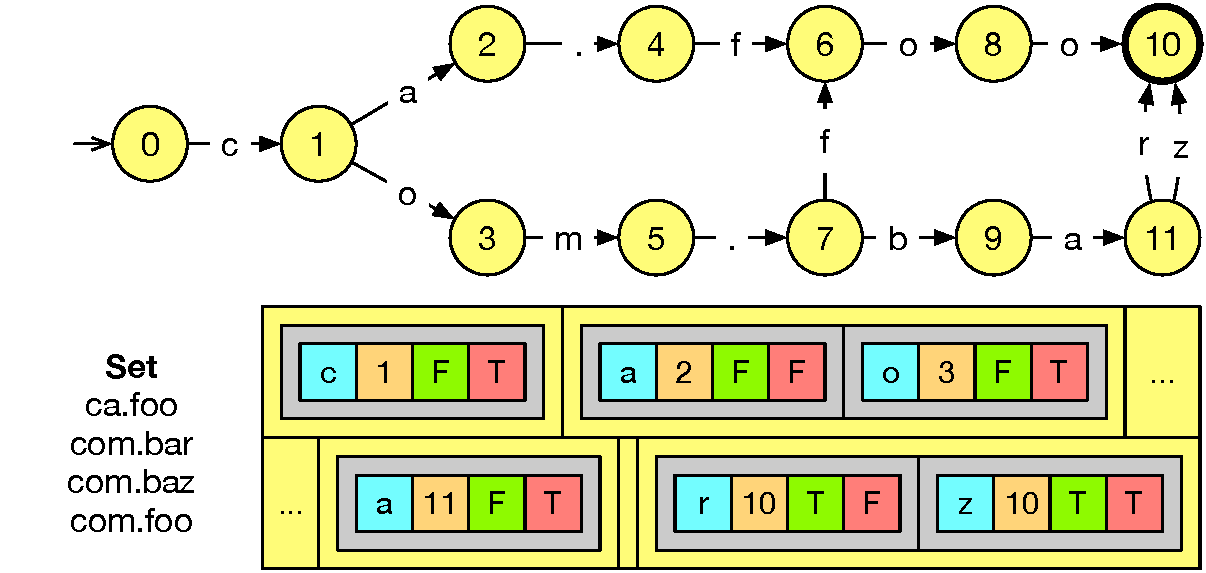
\includegraphics[width=\linewidth]{fig/dafsa}
  \caption{A simple \ac{dafsa} with one-character transitions, along with the
    set of strings it represents and its succinct representation as a vector of
    variable-length bitstrings. In this representation, each edge (gray)
    consists of a label (blue) and next state (orange), along with flags
  indicating whether the next state is an accept state (green) and whether the
edge is the last one outgoing from this state (red).}
  \label{fig:dafsa}
\end{figure}

In our log aggregator prototype, we chose to represent the signaling set as a
data structure known as a \emph{\ac{dafsa}}, which succinctly stores a set of
strings and supports efficient membership queries in this set, and can be
efficiently constructed with minimal size~\cite{daciuk2000incremental}. As shown
in \autoref{fig:dafsa}, \iac{dafsa} takes advantage of both common prefixes and
suffixes that appear in a set of strings; since such patterns are frequent in a
large set of \acp{fqdn}, much of the redundancy in \httpsset can be removed with
this approach. Additionally, \acp{dafsa} can also be represented succinctly,
using the approach we describe below~\cite{daciuk2012smaller}. Given the
characteristics of our input set as described in
\autoref{sec:evaluation:implementation}, we make two additional design
changes to our \ac{dafsa} representation that further reduce its size.

To precisely describe these changes, we begin by presenting a formal framework
to describe \acp{dafsa}. Formally, \iac{dafsa} is a tuple $(\symbols, \states,
\initstate, \transfunc, \finalstates)$ where
\begin{inparaenum}
\item \symbols is a set of possible \emph{input symbols},
\item \states is a set of \emph{states},
\item \initstate is an \emph{initial state} where $\initstate \in \states$,
\item $\transfunc: \states \times \symbols \to \states$ is a partially-defined
  \emph{state transition function} that maps a state-symbol pair to a new state,
  and
\item \finalstates is a set of \emph{accept states} where $\finalstates
  \subseteq \states$.
\end{inparaenum}
We begin by building the \ac{dafsa} as described in previous work, which assumes
single-character transitions~\cite{daciuk2000incremental} as shown in
\autoref{fig:dafsa}. Thus \symbols is the set of ASCII characters allowed in
\acp{fqdn}.

We succinctly represent the \ac{dafsa} as a binary bitvector by following the
high-level approach of previous work~\cite{daciuk2012smaller}. Intuitively, the
\ac{dafsa} can be represented as a vector of state encodings. In turn, the
encoding of a state $s \in \states$ can be represented by
\begin{inparaenum}
\item whether or not the $s \in \finalstates$, and
\item a representation of the state's outgoing transitions.
\end{inparaenum}
By our definition of \transfunc, for a state $s$, if $\transfunc(s, \sigma) =
t$, then each outgoing transition must be represented by an encoding of the
label $\sigma$ and the destination state $t$. While this construction leaves the
exact encoding underspecified, we observe two factors that heavily influence the
size of the final bitvector:
\begin{inparaenum}
\item the overall number of outgoing transitions, and
\item the size of the representation of each transition's label and destination
  state.
\end{inparaenum}
Our design extensions focus on leveraging characteristics of our underlying data
to minimize the size of the \ac{dafsa} representation through these factors.

\begin{figure}
  \centering
  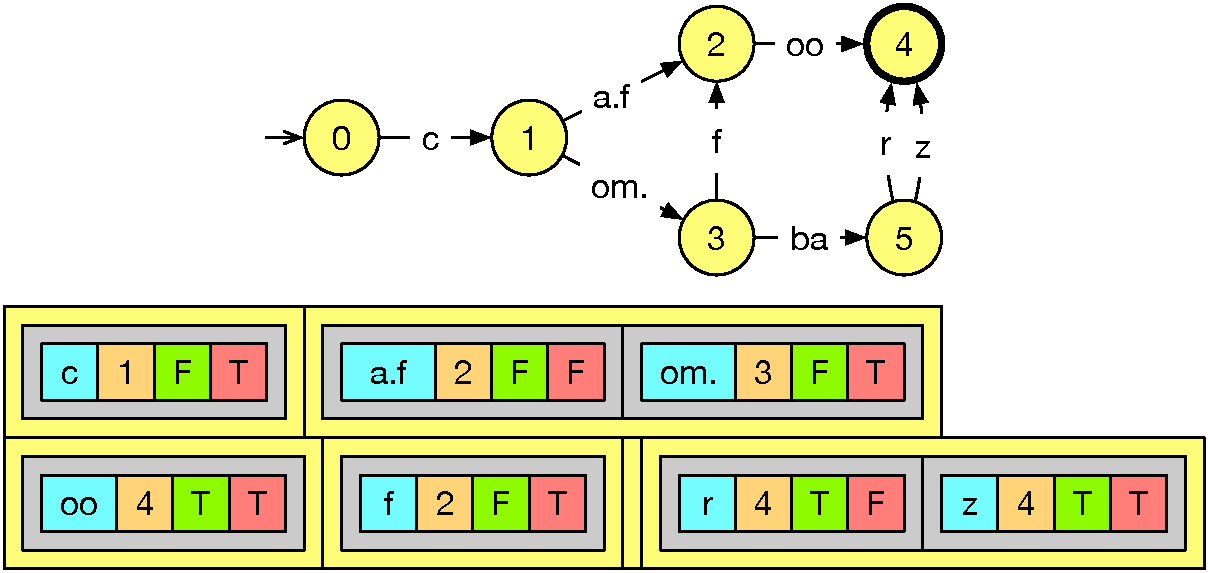
\includegraphics[width=\linewidth]{fig/dafsa_compact}
  \caption{The \ac{dafsa} from \autoref{fig:dafsa} with its long edges
  compacted. The binary representation is more succinct than its counterpart.}
  \label{fig:dafsa_compact}
\end{figure}

The first extension we make to this design is called \emph{path compaction}. In
a nutshell, path compaction removes states with certain properties to reduce the
overall number of edges in the \ac{dafsa}, at the cost of lengthening labels. To
do this, we first transform $(\symbols, \states, \initstate, \transfunc,
\finalstates)$ to $(\symbolstrings, \states, \initstate, \transfunc,
\finalstates)$, where $\symbolstrings = \bigcup_{i=0}^{253} \symbols^i$,
replacing the set of ASCII characters with the set of all strings up to 253
characters in length. We take this as our starting \ac{dafsa} for state
compaction. We then repeatedly select a state $s$ in the current \ac{dafsa} and
transform the \ac{dafsa} to $(\symbolstrings, \states \setminus \{s\},
\initstate, \transfunc', \finalstates)$, where $\transfunc'$ is as we describe
below.

For a state $s$, consider the \emph{incoming transitions} of $s$
\begin{equation*}
  \intrans{s} = \{(t, x) \in \states \times \symbolstrings \mid \transfunc(t, x)
  = s\}
\end{equation*}
and the \emph{outgoing transitions} of $s$
\begin{equation*}
  \outtrans{s} = \{(t, x) \in \states \times \symbolstrings \mid \transfunc(s,
  x) = t\}.
\end{equation*}
In the transformation, we eliminate $s$ by pairwise joining its incoming and
outgoing transitions, thus ``routing'' transitions around $s$. We thus define
$\transfunc'(t, x)$ as follows: for all $(t, x)$ where $t, x) \notin
\intrans{s}$ and $t \ne s$, let $\transfunc'(t, x) = \transfunc(t, x)$, and for
each 4-tuple $(t, u, x, y) \in \intrans{s} \times \outtrans{s}$, let
$\transfunc'(t, x \concat y) = u$.

There are restrictions on which states we can eliminate this way. In particular,
if $s \in \finalstates$, then removing $s$ destroys information and thus $s$
cannot be eliminated from the \ac{dafsa}. If we consider states as nodes in a
graph having an in-degree $\indegree(s) = |\intrans{s}|$ and an out-degree
$\outdegree(s) = |\intrans{s}|$, then we observe that we cannot eliminate $s$ if
$\indegree(s) = 0$ or $\outdegree(s) = 0$, either, because doing so would also
destroy information from the \ac{dafsa}. Finally, we observe that eliminating
$s$ results in a change in the overall number of edges equal to
$\indegree(s)\outdegree(s) - \indegree(s) - \outdegree(s)$, since this
transformation eliminates all incoming and outgoing transitions of $s$ and adds
pairwise transitions. Thus if $\indegree(s) > 1$ and $\outdegree(s) > 1$, then
the overall number of edges does not decrease, since in this case
$\indegree(s)\outdegree(s) > \indegree(s) + \outdegree(s)$.


\subsection{Building the \ac{name} Policy Database}
\label{sec:design:policy}

Determining the key policy
\begin{compactitem}
\item Given a set of currently valid certificate chains for the same public key,
  take the min-cut to find the strength of this key
\item Consider EV certificates separately from non-EV certificates
\item Repeat this for all public keys for a domain, thus forming a $(m, n)$ pair
  for each key where $m$ is the number of EV certs and $n$ the number of
  non-EV certs
\item The key policy is $(x, y)$ where $x$ is the maximum of all $m$ values
  observed and $y$ is the maximum of all $n$ values for that specific $m$ value
\item Any key policy beyond 1 places the domain in \multicertset
\item Revocation
\item Update interval
\end{compactitem}

\subsection{The Extended \ac{tls} Handshake}
\label{sec:design:handshake}


\subsection{Bootstrapping Advanced Policies}
\label{sec:design:bootstrapping}

\begin{compactitem}
\item Use keys established by these key policies to bootstrap more advanced
  policies
\item As an example, use PoliCert (since it has a clean separation between
  policy and certificate)
\end{compactitem}
